%!TEX TS-program = xelatex
\documentclass[]{friggeri-cv}
\usepackage{afterpage}
\usepackage{hyperref}
\usepackage{color}
\usepackage{xcolor}
\hypersetup{
    pdftitle={},
    pdfauthor={},
    pdfsubject={},
    pdfkeywords={},
    colorlinks=false,       % no lik border color
   allbordercolors=white    % white border color for all
}
\addbibresource{bibliography.bib}
\RequirePackage{xcolor}
\definecolor{pblue}{HTML}{0395DE}

\begin{document}
\header{Victor}{Huesca}
      {Étudiant en Informatique}
      
% Fake text to add separator      
\fcolorbox{white}{gray}{\parbox{\dimexpr\textwidth-2\fboxsep-2\fboxrule}{%
.....
}}

% In the aside, each new line forces a line break
\begin{aside}
    ~~~
  \section{Adresse}
    27 Impasse Aussel,
    34660 Cournonterral, France
    ~
  \section{Courriel}
    \href{mailto:victor.huesca@etu.umontpellier.fr}{victor.huesca@\\\textit{etu.umontpellier.fr}}
    ~
  \section{Téléphone}
    \numero +33 651 721 065
    ~
  \section{Gits}
    \href{https://github.com/Victor333Huesca}{GitHub\textit{/Victor-Huesca}}
    \href{https://gitlab.info-ufr.univ-montp2.fr/u/e20150002352}{GitLab\textit{/Victor-Huesca}}
    ~
  \section{Programmation}
    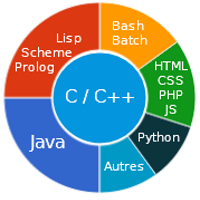
\includegraphics[scale=0.66]{img/prog.png}
    ~
  \section{OS Favoris}
    \textbf{Windows}
\includegraphics[scale=0.40]{img/5stars.png}
    \textbf{GNU/Linux}
\includegraphics[scale=0.40]{img/4stars.png}
    \textbf{Android}
\includegraphics[scale=0.40]{img/3stars.png}
    \textbf{MacOS}
\includegraphics[scale=0.40]{img/1stars.png}
    ~
  \section{Compétences Personnelles}
    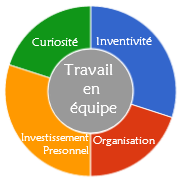
\includegraphics[scale=0.75]{img/personal.png}
    ~
  \section{Langues Parlées}
    \textbf{Français}
\includegraphics[scale=0.40]{img/5stars.png}
    \textbf{Anglais}
\includegraphics[scale=0.40]{img/4stars.png}
    \textbf{Anglais}
\includegraphics[scale=0.40]{img/2stars.png}
\end{aside}

\section{Expériences}
\begin{entrylist}
  \entry
    {2016}
    {Stage dans la fonction publique}
    {\href{http://www.montpellier.fr/}{Mairie de Montpellier}}
    {Stage d'un mois à la Direction des Systèmes d'Information au sein du pôle éducation numérique de la mairie de Montpellier. Remise à niveau des postes élèves des écoles de Montpellier.\\}
  \entry
    {2013 - 2015}
    {Cours de soutien}
    {A domicile}
    {Dispence de cours cours de soutien et d'aide aux devoirs à des élèves de la 6ème à la terminale.\\}
  \entry
    {2012}
    {Stage en entreprise}
    {Boulangerie - St Georges d'Orques}
    {Stage au sein de la boulangerie / pâtisserie "Au plaisirs de St Georges".\\Stage d'observation majoritairement et confection de quelques produits basiques.\\}
\end{entrylist}

\section{Formation}
\begin{entrylist}
  \entry
    {2016}
    {License 2 Informatique CMI}
    {\href{http://sciences.edu.umontpellier.fr/}{Université de Montpellier}}
    {Etudes d'informatiques en Cursus Master Ingégnerie à l'université de Montpellier 2.\\}
  \entry
    {2015}
    {Baccalauréat Scientifique}
    {Lycée Général Jean Mermoz}
    {Baccalauréat en Sciences de l'Ingénieur spécialité mathématiques obtenu avec la mention Assez Bien.\\}
  \entry
    {2013}
    {BIA}
    {Lycée Jean Monnet}
    {Brevet d'Initiation à l'Aéronautique (diplôme national).\\}
  \entry
    {2012}
    {Brevet des Collèges}
    {Collège François Rabelais}
    {Obtenu avec la mention Bien.\\}
\end{entrylist}

\section{Compétences}
\begin{itemize}
  \item Logiciels Bureautique (Suite Office, \LaTeX).
  \item Programmation
  \item Web
\end{itemize}
~
\section{Centres d'Intérêt}
\begin{itemize}
  \item Sciences (Formelles, Physiques, Sociales, Appliquées)
  \item Sports (Volley-ball, Badminton, Tennis, ...)
  \item Autres (Musique, Lecture, Pâtisserie)
\end{itemize}


%%% This piece of code has been commented by Karol Kozioł due to biblatex errors. 
% 
%\printbibsection{article}{article in peer-reviewed journal}
%\begin{refsection}
%  \nocite{*}
%  \printbibliography[sorting=chronological, type=inproceedings, title={international peer-reviewed conferences/proceedings}, notkeyword={france}, heading=subbibliography]
%\end{refsection}
%\begin{refsection}
%  \nocite{*}
%  \printbibliography[sorting=chronological, type=inproceedings, title={local peer-reviewed conferences/proceedings}, keyword={france}, heading=subbibliography]
%\end{refsection}
%\printbibsection{misc}{other publications}
%\printbibsection{report}{research reports}

\end{document}
